\documentclass[%
 reprint,
 amsmath,amssymb,
 aps,
 10pt
]{revtex4-2}
\usepackage{graphicx}% Include figure files
\usepackage[version=4]{mhchem}
\usepackage{dcolumn}% Align table columns on decimal point
\usepackage{bm}% bold math
\usepackage{siunitx}
\usepackage{lmodern}
\showthe\columnwidth
\usepackage[mathlines]{lineno}% Enable numbering of text and display math
\makeatletter
\providecommand\add@text{}
\newcommand\tagaddtext[1]{%
  \gdef\add@text{#1\gdef\add@text{}}}% 
\renewcommand\tagform@[1]{%
  \maketag@@@{\llap{\add@text\quad}(\ignorespaces#1\unskip\@@italiccorr)}%
}
\makeatother

\begin{document}
\begin{abstract}
	Measuring the Sun is important for understanding the ways that stars function, and allows us to make similar measurements for starts that are much further away. One important characteristic is the temperature of the sun $T_\odot$. Ensuring high-precision measurements of this value are paramount to the field of stellar astronomy. This study sought out to find the effectiveness of measuring $T_\odot$ in a fashion different than is currently accepted within literature. We found a measurement of $T_\odot = \SI{4897.9}{\kelvin} \pm 12.5$ K, suggesting that this method should not be adopted by the field for determining $T_\odot$.
\end{abstract}
\preprint{AAPM/123-QED}
\title[title]{Monochromatic method for determining $T_\odot$.}
\author{Parker Wise$^{1}$ and Dayne Locke$^{1}$\\$^{1}$University of Kansas}
\date{April 2025}
\maketitle
\showthe\textwidth
\section{Introduction}
The Sun is of particular interest because it is the closest star. Investigation of the properties of the Sun allow for a deeper understanding of stars. One particularly important variable is the Sun's temperature. The temperature of the Sun is directly related to the luminosity of the sun. 
\subsection{Black Bodies}
A black body is a hypothetical body that absorbs all incident light. At equilibrium, this means that any and all radiation that exits the black body are due to thermal radiation. Stars act as great approximations of black bodies. As such, the various equations that describe black bodies can be applied to stars including the Sun. 
\par
The radiant flux of a black body, $j^*$, can be modeled with the Stefan-Boltzmann Law \citep{Stefan:1879txg},
\begin{equation}
	j^{*} = \sigma T^4,\tagaddtext{[\unit{\watt\per\meter\squared}]}
	\label{stefan-boltzman law}
\end{equation}
where $\sigma$ is the Stefan-Boltzmann constant and $T$ is the temperature of the black body.
\par
Black bodies do not emit equally at all wavelengths of light as can be seen in figure \ref{blackbody spectra}. The energy emitted by a black body as a function of observed wavelength can be describe by Wien's Approximation \citep{wein_1896},
\begin{equation}
	E_\lambda = C_1 \lambda^{-5}\exp{(-C_2/\lambda T)},
	\label{wien approx}
\end{equation}
where $C_1 = 2\pi h c^2 = \SI{3.74e-16}{\watt\per\meter\squared}$ and $C_2 = hc/k = \SI{1.44e-2}{\meter\kelvin}$.
\par
Using equation \ref{wien approx}, the temperature of two objects can be compared by observing emitted energies at one wavelength,
\begin{equation}
	\left(\frac{1}{T_1} - \frac{1}{T_2}\right) = \frac{\lambda}{C_2}\ln \left(\frac{E_2}{E_1}\right).
	\label{wien ratio}
\end{equation}
This equation is the basis by which optical pyrometry is done.
\subsection{Radiometry}
Radiometry is the practice of measuring the intensity of light. In radiometry, the tool used for finding the temperature of an object is a pyrometer. Optical pyrometers function by comparing the temperature of a known source to the temperature of a source you are attempting to measure by utilizing equation \ref{wien ratio} \citep{gilchrist_fuels_1977}. The specifics of the instrument used in this experiment will be discussed in more detail in section \ref{methods}.
\par
\begin{figure*}
	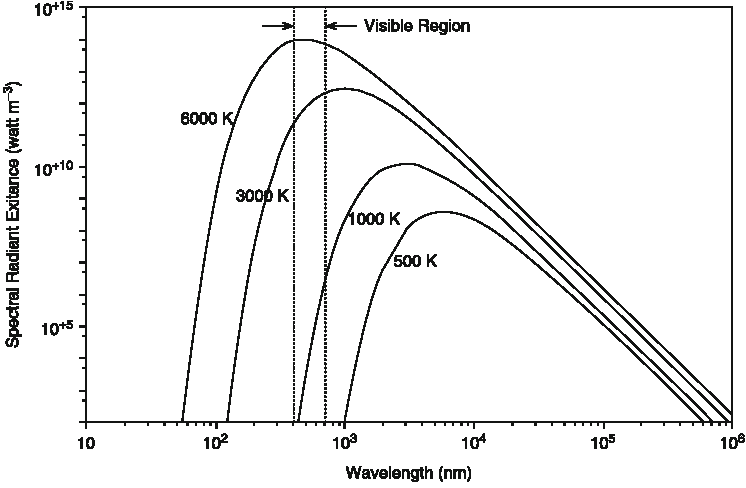
\includegraphics{blackbody.pdf}
	\caption{\label{blackbody spectra} Black body spectra. The shape of the black body spectra for bodies at varying temperatures.
	\citep{luo_blackbody_2015} }
\end{figure*}
\subsection{Calculation of $T_\odot$}
The accepted value for the temperature of the sun $T_\odot$, by the International Astronomical Union (IAU) is found using the Stefan-Boltzmann's law with the best estimates for the solar photospheric radius $R_\odot$, the astronomical unit, and the total solar irradiance $S_\odot$ \citep{prsa_nominal_2016}
. $S_\odot$ is the mean total electromagnetic radiation from the sun, integrated across all wavelengths. $S_\odot$ is measured using an absolute cavity radiometer \citep{kendall_primary_1969}. One of the largest differences between the absolute cavity radiometer and a pyrometer is that the radiometer measures the intensity of light, whereas a pyrometer "interprets" the measured intensity and reads out a temperature.
\subsection{Radiative Transfer}
As light travels through a medium it undergoes the process of radiative transfer. Light from the Sun is absorbed as it travels through the atmosphere. The way that the intensity of light $I_\lambda$ is affected by this absorption can be modeled using Beer's Law \citep{petty_first_2006},
\begin{equation}
	\log{(I_\lambda)} = -\frac{\tau_\lambda}{\mu}+\log{(S_\lambda)},
	\label{beers law}
\end{equation}
where $\tau_\lambda$ is the optical depth of the atmosphere, $S_\lambda$ is the intensity of the sun, $\mu = \cos(\theta)$ and $\theta$ is the solar zenith angle.
\par
This study seeks to look at a monochromatic ground-based determination of $T_\odot$ through the use of an optical pyrometer. The results of this study will inform us on the effectiveness of this method in comparison to the currently accepted method.
\section{Methods}\label{methods}
\begin{figure*}
	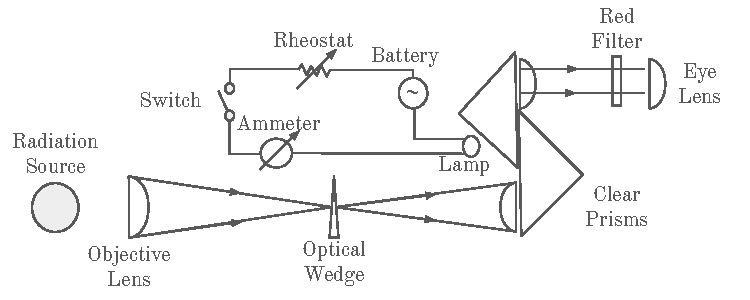
\includegraphics{setup.pdf}
	\caption{\label{app} Experimental Apparatus.
	Incoming radiation is focused by the objective lens. Then using an optical wedge the operator is able to lower the intensity of light. The operator manipulates the optical wedge until the incoming light matches intensity with an internal lamp with a known temperature. The instrument then reads out a measured temperature.
	}
\end{figure*}
The schematic for the apparatus used within this experiment can be seen in figure \ref{app}. The apparatus is housed within a hand held instrument. In order to collect data we first had to point the instrument at the sun. At this point, a filter was added that allowed for us to read higher temperatures.
\par
In addition, a post hoc filter was added to the instrument that increased every temperature read out by about 3000 K. Without the second filter, it would not have been possible to collect a temperature for an object as hot as the Sun. 
\par
Measurements were taken for a variety of times throughout the day to see how a differing airmass, and by extension, the atmosphere, would affect the measurement.
\section{Results}
Figure \ref{temps} shows measurements taken of $T_\odot$ at varying points in the day. We end up with an average $\bar{T}_\odot = SI{4897.9}{\kelvin} \pm 12.5$ K.
The results show a large range of temperatures that are not within uncertainty of each other. The plot also shows a rise, and subsequent fall, in the temperature readings around midday. The variation in time of day cooresponds to differing solar zenith angles, and thus, differing airmasses. This shows that atmospheric extinction has a non-negligible impact on temperature readings.
\par
Since there were no calculations done other than averaging for this experiment, there is no need to propagate uncertainty. The uncertainty of our measurements were half the distance between each tick on the pyrometers readout, which cooresponds to 12.5 K.  
\begin{figure*}
	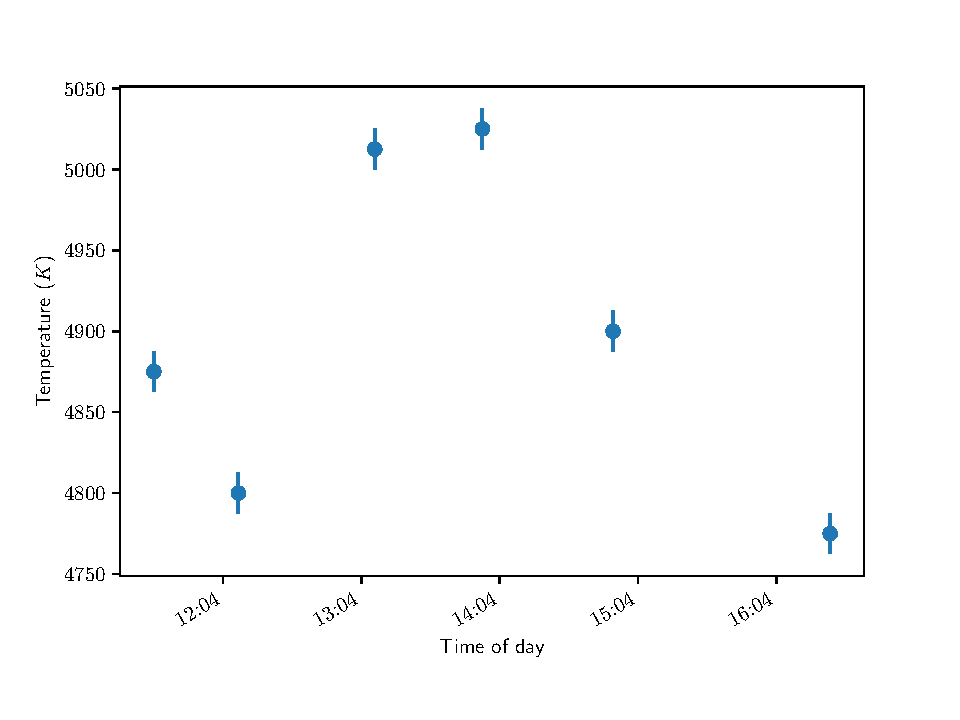
\includegraphics{../python/temps.pdf}
	\caption{\label{temps} Measured $T_\odot$ at varying times of day. 6 data points were taken at roughly one-hour intervals and can be seen in the figure in blue.}
\end{figure*}
\section{Conclusions}
The results from this study vary largely from widely accepted values of $T_\odot$. The IAU's nominal value for $T_\odot$ is $\SI{5772}{\kelvin}$. Several factor play into why the nominal value falls outside of uncertainty of $\SI{4897.9}{\kelvin} \pm$ 12.5 K.
\par
One possible reason could be due to the instrument itself. Pyrometers can only calculate a valid temperature when the object being measured takes up the entire field of view. With the instrument used in the experiment, at the highest level of magnification, the Sun did not take up the entire field of view. The reason this matters is because the Pyrometer itself does not actually account for distance. The way that it compensates has to do with the fact that both solid angle and radiant flux fall off as $r^{-2}$. Ensuring that the object takes up the whole field of view allows for these two values to cancel each other out. 
\par
Another possible source of error could be the atmospheric extinction. As light travels through the atmosphere some of it is absorbed. Without accounting for this, it will appear that the Sun is colder than it really is. As we saw in figure \ref{temps}, it appears that atmospheric extinction does play a large role in output temperature reading. By using equation \ref{beers law}, a fit could be done to solve for $\T_\lambda$ and $S_\lambda$, but that would defeat the point of using a pyrometer rather than a radiometer, seeing is it would require us to convert our temperature readings into intensities, and one of the major draws to using a pyrometer rather than a radiometer is the fact that it directly reads out temperature instead of radiant flux.
\par
A final source of error could be the monochromatic nature of the instrument. The pyrometer used in this experiment measures light at $\SI{655}{\nano\meter}$, whereas the sun's spectra peaks at around $\SI{500}{\nano\meter}$, this also suggests a lower temperature than what we've previously measured. 
\par
In all, the results of this experiment suggest that this method of calculating the temperature of the Sun is quite flawed. With the use of a radiometer that reads bolometric intensity, many of the issues found in this experiment could be solved.
\section{Improvements from first draft}
Within this draft, more data points taken and were plotted with uncertainty. More detail and theory was given to atmospheric extinction. Most of the sections were edited in some way as to make the point come across clearer.
\bibliography{sources}
\bibliographystyle{prl}
\end{document}
